\section{El kernel Linux}
\subsection{Funcionamiento del kernel Linux}
\subsubsection{Administraci'on del Procesador}
Linux es un sistema operativo que permite la multitarea o multiprogramaci'on, es por esto que en el n'ucleo existe una funci'on que se encarga de la organizaci'on de los procesos. En el transcurso de la ejecuci'on un proceso en Linux puede pasar por cinco estados diferentes. Estos estados son:

\begin{itemize}
	\item En ejecuci'on: el proceso es ejecutado por el procesador.
	\item A punto: el proceso podr'ia ser ejecutado pero otro proceso se est'a ejecutando en ese momento.
	\item Suspendido: el proceso est'a en espera de un recurso.
	\item Parado: el proceso ha sido suspendido por una intervenci'on externa.
	\item Zombi: el proceso ha terminado su ejecuci'on pero sigue siendo referenciado en el sistema.
\end{itemize}

Los atributos que el sistema mantiene mientras un proceso se esta ejecutando son: el estado, el valor de los registros, la identidad del usuario que lo ejecuta, la informacion utilizada por el n'ucleo para proceder al ordenamiento de los procesos (prioridad), la informaci'on respecto del espacio de direccionamiento del proceso (segmentos de c'odigo, de datos, de pila), informaci'on respecto a las entradas/salidas efectuadas por el proceso e informaci'on que resume los recursos utilizados por el proceso.
La forma que posee Linux para ejecutar varios procesos es muy parecida a la que poseen los dem'as sistemas operativos que admiten la multiprogramaci'on. El sistema mantiene una lista de procesos \emph{a punto} que podr'ia ejecutar y procede peri'odicamente a un ordenamiento. A cada proceso se le atribuye un lapso de tiempo. Linux elige un proceso a ejecutar, y le deja ejecutarse durante ese lapso. Cuando ha transcurrido, el sistema hace pasar al proceso actual al estado \emph{a punto}, y elige otro proceso que ejecuta durante otro lapso. El lapso de tiempo es muy corto y el usuario tiene la impresi'on que varios procesos se ejecutan simultaneamente, aunque s'olo un proceso se ejecuta en un instante dado. Se dice que los procesos se ejecutan en pseudoparalelismo.
La funci'on del n'ucleo que decide qu'e proceso debe ser ejecutado por el procesador es el Coordinador. 'este explora la lista de procesos \emph{a punto} y utiliza varios criterios para elegir el proceso a ejecutar. El coordinador de L'inux proporciona tres pol'iticas de coordinaci'on diferentes: una para los procesos "normales" y dos para los procesos de "tiempo real".
A cada proceso se le asocia un tipo de proceso, una prioridad fija y una prioridad variable. El tipo de proceso puede ser:

\begin{itemize}
	\item SCHED\_FIFO para un proceso de tiempo real no peemtivo.
	\item SHCED\_RR para un proceso de tiempo real peemtivo.
	\item SCHED\_OTHER para un proceso cl'asico
\end{itemize}

La pol'itica de coordinaci'on depende del tipo de procesos contenidos en la lista de procesos a punto de ejecutar:
Cuando un proceso de tipo SCHED\_FIFO est'a \emph{a punto}, se ejecuta inmediatamente. El coordinador prioriza la elecci'on del proceso de tipo SCHED\_FIFO que posea la m'as alta prioridad, y lo ejecuta. Este proceso no es normalmente preemtible, es decir, que posee el procesador, y el sistema s'olo interrumpir'a su ejecuci'on en tres casos:

\begin{itemize}
	\item Otro proceso de tipo SCHED\_FIFO que posea una prioridad m'as elevada pasa al estado \emph{a punto}.
	\item El proceso se suspende en espera de un evento, como por ejemplo el fin de una entrada/salida.
	\item El proceso abandona voluntariamente el procesador por una llamada a la primitiva \texttt{sched\_yield}. El proceso pasa al estado \emph{a punto} y se ejecutan otros procesos.
\end{itemize}

Cuando un proceso de tipo SCHED\_RR est'a a punto, se ejecuta inmediatamente. Su comportamiento es similar al de un proceso de tipo SCHED\_FIFO, con una excepci'on: cuando el proceso se ejecuta, se le atribuye un lapso de tiempo. Cuando este lapso expira, puede elegirse y ejecutarse un proceso de tipo SCHED\_FIFO o SCHED\_RR de prioridad superior o igual a la del proceso actual.
Los procesos de tipo SCHED\_OTHER 'unicamente pueden ejecutarse cuando no existe ning'un proceso de "tiempo real" en estado \emph{a punto}. El proceso a ejecutar se elige tras examinar las prioridades din'amicas. La prioridad din'amica de un proceso se basa por una parte en el nivel especificado por el usuario por las llamadas al sistema nice y setpriority, y por otra parte en una variaci'on calculada por el sistema. Todo proceso que se ejecuta durante varios ciclos de reloj disminuye en prioridad y puede as'i llegar a ser menos prioritario que los procesos que no se ejecutan, cuya prioridad no se ha modificado.
Como se puede observar todo el peso de la planificaci'on de la ejecuci'on de los procesos en Linux la lleva a cabo el Coordinador.

\subsubsection{Administraci'on de Memoria}
Linux tambi'en maneja la gesti'on de memoria. Este sistema utiliza la memoria p'aginada por demanda (tambi'en conocida como paginada con intercambio) adem'as de segmentaci'on. La raz'on por la cual se utiliza este modo de gesti'on de memoria m'as complejo pero tambi'en completo es porque este sistema operativo debe ser capaz de poder ejecutar, entre otras muchas cosas, el entorno gr'afico Xwindows, adem'as de dar soporte a la multiprogramaci'on y multiusuario. Si unimos todo esto es f'acil pensar que los programas a ejecutar pueden ser mayores que el tama�o de la memoria y que debido a tener soporte multiusuario los procesos en ejecuci'on pueden ser muchos. Para realizar el intercambio Linux no s'olo lo har'a con el disco duro sino que como veremos m'as adelante ser'a capaz de gestionar unos dispositivos llamados swap que no tienen porqu'e ser el disco duro.
Para poder entender totalmente la gesti'on que Linux realiza de la memoria veremos una explicaci'on detallada de como se pagina y se gestiona la memoria.
\paragraph{Protecci'on de zonas de memoria}
Al estar cargados en memoria varios procesos, se pueden producir problemas en cuanto a la protecci'on de las zonas de memoria. Para solucionar este problema Linux utiliza la segmentaci'on para separar las zonas de memoria asignadas al n'ucleo y a los procesos. Los segmentos se refieren a los tres primeros Gigabytes de espacio de direccionamiento de los procesos y su contenido pueden leerse y modificarse en modo usuario. El cuarto Gigabyte del espacio de direccionamiento y su contenido s'olo puede leerse y modificarse en modo n'ucleo. De esta forma el c'odigo y los datos del n'ucleo quedan totalmente protegidos.
\paragraph{Paginaci'on}
Linux utiliza los mecanismos de memoria virtual proporcionados por el procesador sobre el que se ejecuta. Las direcciones manipuladas por el n'ucleo y los procesos son direcciones virtuales y el procesador efect'ua una conversi'on para transformar una direcci'on virtual en direcci'on f'isica en memoria central.
El mecanismo de conversi'on es el siguiente: una direcci'on de memoria se descompone en dos partes, un n'umero de p'agina y un desplazamiento en la p'agina. El n'umero de p'agina se utiliza como 'indice en una tabla, llamada tabla de p'aginas, lo que proporciona una direcci'on f'isica de p'agina en memoria central. A esta direcci'on se le a�ade el desplazamiento para obtener la direcci'on f'isica de la palabra de memoria en concreto.
Debido al tama�o del espacio de memoria direccionable por los procesadores, la tabla de p'aginas raramente se implementa en forma de una sola tabla contigua en memoria. Como la tabla de p'aginas debe ser residente en memoria, necesitar'ia un exceso de memoria para esta tabla. Por esta raz'on la tabla de p'aginas a menudo se descompone en varios niveles, con un m'inimo de 2.
%En el siguiente dibujo se puede observar esta descomposici'on.

%\begin{figure}[h]
%\centering
%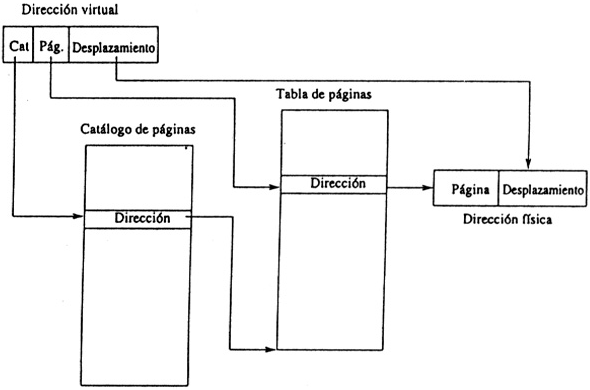
\includegraphics[scale=0.5]{imagememory.png}
%\end{figure}

El inter'es de esta tabla de p'aginas por niveles se basa en que la tabla de p'aginas no necesita cargarse completamente en memoria.
Linux gestiona la memoria central y las tablas de p'aginas utilizadas para convertir las direcciones virtuales en direcciones f'isicas. Implementa una gesti'on de memoria que es ampliamente independiente del procesador sobre el que se ejecuta.
En realidad, la gesti'on de la memoria implementada por Linux considera que dispones de una tabla de p'aginas a tres niveles:

\begin{enumerate}
	\item la tabla global, cuyas entradas contienen las direcciones de p'aginas que contienen tablas intermedias;
	\item las tablas intermedias, cuyas entradas contienen las direcciones de p'aginas que contienen tablas de p'aginas;
	\item las tablas de p'aginas, cuyas entradas contienen las direcciones de p'aginas de memoria que contienen el c'odigo o los datos utilizados por el n'ucleo o los procesos de usuario.
\end{enumerate}

Ya que posee esta paginaci'on Linux intenta sacarle el m'aximo partido y cuando varios procesos acceden a los mismos datos Linux intenta compartir al m'aximo las p'aginas. Por ejemplo, si varios procesos ejecutan el mismo programa, el c'odigo del programas se carga una sola vez en memoria, y las entradas de las tablas de p'aginas de los diferentes procesos apuntan a las mismas p'aginas de memoria.
Adem'as, Linux implementa una t'ecnica de copia en escritura, que permite minimizar el n'umero de p'aginas de memoria utilizadas. Cuando se crea un procesos, llamando a fork, hereda el espacio de direccionamiento de su padre. Evidentemente, el segmento de c'odigo no se duplica, pero Linux tampoco duplica el segmento de datos. Al duplicar el proceso, todas las p'aginas del segmento de datos s marcan como accesibles en lectura exclusiva en las tablas de p'aginas de los dos procesos. Cuando uno de los dos procesos intenta modificar un dato, el procesador provoca una interrupci'on de memoria, que gestiona el n'ucleo. Al tratar esta interrupci'on, Linux duplica la p'agina afectada y la inserta en la tabla de p'aginas del proceso que ha causado la interrupci'on.
\paragraph{Intercambio (Gesti'on de dispositivos Swap)}
Bajo Linux, todo dispositivo en modo bloque o archivo regular puede usarse como dispositivo de swap. El n'ucleo de Linux guarda en memoria una lista de dispositivos de swap activos. Se utiliza una tabla de descriptores, el la que cada uno describe un despositivo de swap.
Cuando una p'agina se escribe en un dispositivo de swap, se le atribuye una direcci'on. Esta direcci'on combina el n'umero de dispositivo de swap y el 'indice de la p'agnia utilizada en el dispositivo. Cuando una p'agina debe descargarse de la memoria, se le asigna una p'agina en un dispositivo de swap, y la direcci'on de dicha p'agina se memoriza para que Linux pueda recargar la p'agina ulteriormente. En lugar de utilizar una tabla que establezca una correspondencia entre las direcciones de p'aginas de memoria y las direcciones de entradas de swap, Linux utiliza un m'etodo original:

\begin{itemize}
    \item Cuando una p'agina de memoria se descarta, la direcci'on de la entrada de swap asignada se guarda en la tabla de p'aginas, en lugar de la direcci'on f'isica de la p'agina. Esta direcci'on est'a concebida para indicar al procesador que la p'agina no est'a presente en memoria.
    \item Cuando se efect'ua un acceso de memoria sobre una p'agina que se ha guardado en un dispositivo de swap, el procesador detecta que la p'agina no est'a presente en memoria y desencadena una interrupci'on. Al tratar esta interrupci'on, Linux extrae la direcci'on de entrada de swap de la entrada correspondiente de la tabla de p'agnias, y utiliza esta direcci'on para localizar la p'agina en el swap y cargarla.
\end{itemize}

\paragraph{Asignaci'on de Memoria}
Hasta el momento hemos visto como Linux utiliza una memoria paginada y unos elementos para poder realizar una utilizaci'on 'optima de la memoria pero no hemos hablado de qu'e algoritmo o estrategia utiliza para asignar la memoria. Para llevar la cuenta de como est'a la memoria en cada momento Linux no utiliza una lista simple, Linux utiliza el principio del Buddy system. Su principio es bastante simple: el n'ucleo mantiene una lista de grupos de p'aginas. Estos grupos son de tama�o fijo y se refieren a p'aginas contiguas en memoria.
El principio b'asico del Buddy system es el siguiente: para cada petici'on de asignaci'on, se usa la lista no vac'ia que contiene los grupos de p'aginas de tama�o inmediatamente superior al tama�o especificado, y se selecciona un grupo de p'aginas de esta lista. Este grupo se descompone en dos partes: las p'aginas correspondientes al tama�o de memoria especificado, y el resto de p'aginas que siguen disponibles. Este resto puede insertarse en las otras listas.
Al liberar un grupo de p'aginas, el n'ucleo intenta fusionar este grupo con los grupos disponibles, a fin de obtener un grupo disponible de tama�o m'aximo.
Para simplificar la asignaci'on y liberaci'on de un grupo de p'aginas, el n'ucleo s'olo permite designar grupos de p'aginas cuyo tama�o sea predeterminado y corresponda a los tama�os gestionados en las listas.
Como vemos este m'etodo es un poco complicado pero con este m'etodo se permite una mejor utilizaci'on de la memoria.
